\documentclass[sigconf]{acmart}

%%
%% \BibTeX command to typeset BibTeX logo in the docs
\AtBeginDocument{%
  \providecommand\BibTeX{{%
    \normalfont B\kern-0.5em{\scshape i\kern-0.25em b}\kern-0.8em\TeX}}}

%% Rights management information.  This information is sent to you
%% when you complete the rights form.  These commands have SAMPLE
%% values in them; it is your responsibility as an author to replace
%% the commands and values with those provided to you when you
%% complete the rights form.
%\setcopyright{acmcopyright}
%\copyrightyear{2018}
%\acmYear{2018}
%\acmDOI{10.1145/1122445.1122456}

%% These commands are for a PROCEEDINGS abstract or paper.
\acmConference[Woodstock '18]{Woodstock '18: ACM Symposium on Neural
  Gaze Detection}{June 03--05, 2018}{Woodstock, NY}
\acmBooktitle{Woodstock '18: ACM Symposium on Neural Gaze Detection,
  June 03--05, 2018, Woodstock, NY}
\acmPrice{15.00}
\acmISBN{978-1-4503-9999-9/18/06}

\usepackage{listings}

%%
%% Submission ID.
%% Use this when submitting an article to a sponsored event. You'll
%% receive a unique submission ID from the organizers
%% of the event, and this ID should be used as the parameter to this command.
%%\acmSubmissionID{123-A56-BU3}

%%
%% The majority of ACM publications use numbered citations and
%% references.  The command \citestyle{authoryear} switches to the
%% "author year" style.
%%
%% If you are preparing content for an event
%% sponsored by ACM SIGGRAPH, you must use the "author year" style of
%% citations and references.
%% Uncommenting
%% the next command will enable that style.
%%\citestyle{acmauthoryear}

%%
%% end of the preamble, start of the body of the document source.

\begin{document}

%%
%% The "title" command has an optional parameter,
%% allowing the author to define a "short title" to be used in page headers.
%% \title{Smart Assignment System for Data Science Education}

\title{An Experimental Study of Memory Management in Rust Programming for Big Data Processing}


% \author{Lars Th{\o}rv{\"a}ld}
% \affiliation{%
%  \institution{The Th{\o}rv{\"a}ld Group}
%  \streetaddress{1 Th{\o}rv{\"a}ld Circle}
%  \city{Hekla}
%  \country{Iceland}}
% \email{larst@affiliation.org}

\author{Shinsaku Okazaki}
\affiliation{%
  \institution{Boston University}
}
\email{so4639@bu.edu}


\author{Kia Teymourian}
\affiliation{%
  \institution{Boston University}
}
\email{kiat@bu.edu}





% Other good conference for publising this idea 

% https://iticse.acm.org/2020/




%%
%% The abstract is a short summary of the work to be presented in the
%% article.
\begin{abstract}

Planning optimized memory management is critical for Big Data analysis tools to
perform faster runtime and efficient use of computation resources.
Modern Big Data analysis tools use application languages that abstract their
memory management so that developers do not have to pay extreme attention
to memory management strategies.

Many existing modern cloud-based data processing systems such as Hadoop, Spark or Flink use
Java Virtual Machine (JVM) and taking full advantage of features such as automated memory management in JVM
including Garbage Collection (GC) which may lead to a significant overhead.
Dataflow-based systems like Spark allow programmers to define complex objects in a
host language like Java to manipulate and transfer tremendous amount of data.

Planning optimized memory management is critical for Big Data analysis tools to
perform faster runtime and efficient use of computation resources.
Modern Big Data analysis tools use application languages that abstract their
memory management so that developers do not have to pay extreme attention
to memory management strategies.

Many existing modern cloud-based data processing systems such as Hadoop, Spark or Flink use
Java Virtual Machine (JVM) and taking full advantage of features such as automated memory management in JVM
including Garbage Collection (GC) which may lead to a significant overhead.
Dataflow-based systems like Spark allow programmers to define complex objects in a
host language like Java to manipulate and transfer tremendous amount of data.
\end{abstract}

%%
%% The code below is generated by the tool at http://dl.acm.org/ccs.cfm.
%% Please copy and paste the code instead of the example below.
%%
%\begin{CCSXML}
%<ccs2012>
% <concept>
%  <concept_id>10010520.10010553.10010562</concept_id>
%  <concept_desc>Computer systems organization~Embedded systems</concept_desc>
%  <concept_significance>500</concept_significance>
% </concept>
% <concept>
%  <concept_id>10010520.10010575.10010755</concept_id>
%  <concept_desc>Computer systems organization~Redundancy</concept_desc>
%  <concept_significance>300</concept_significance>
% </concept>
% <concept>
%  <concept_id>10010520.10010553.10010554</concept_id>
%  <concept_desc>Computer systems organization~Robotics</concept_desc>
%  <concept_significance>100</concept_significance>
% </concept>
% <concept>
%  <concept_id>10003033.10003083.10003095</concept_id>
%  <concept_desc>Networks~Network reliability</concept_desc>
%  <concept_significance>100</concept_significance>
% </concept>
%</ccs2012>
%\end{CCSXML}

%\ccsdesc[500]{Computer systems organization~Embedded systems}
%\ccsdesc[300]{Computer systems organization~Redundancy}
%\ccsdesc{Computer systems organization~Robotics}
%\ccsdesc[100]{Networks~Network reliability}

%%
%% Keywords. The author(s) should pick words that accurately describe
%% the work being presented. Separate the keywords with commas.
% \keywords{datasets, neural networks, gaze detection, text tagging}


%%
%% This command processes the author and affiliation and title
%% information and builds the first part of the formatted document.
\maketitle

\section{Introduction}

Multiple cluster computing analysis tools have been developed, such as Hadoop MapReduce \cite{ApacheHadoopHomePage}, 
Apache Spark \cite{ApacheSparkHomePage}, and Apache Flink \cite{ApacheFlinkHomePage} \cite{DBLP:journals/debu/CarboneKEMHT15}. 
These tools have brought reliable and scalable ways to deal massive data. 
These has become widely popular, in which data-parallel computations are executed on clusters of unreliable machines by systems that automatically provide locality-aware scheduling, 
fault tolerance, and load balancing. 

These tools are constructed on top of Java Virtual Machine (JVM). JVM abstracts hardware and memory management from the developer so that the development is fairly easy. 
In addition, Java or Scala compiled code is platform-independent, which can run on any machine with JVM. However, these advantages may be really critical weakness when it comes to 
processing big data. JVM abstract away most detail regarding memory management from the system designer, including memory deallocation, reuse, and movement, as well as pointers, 
object serialization and deserialization. Since managing and utilizing memory is one of the most important factors determining Big Data systems' performance, 
reliance on a managed environment can mean an order-of-magnitude increase in CPU cost for some computations. This cost may be unacceptable for high-performance tool development by an expert.

To overcome these problems, one can use programming languages with more control on hardware, system languages, for development of Big Data tools. For example, C++ is a general-purpose, statically typed, 
compiled programming language which supports multiple programming paradigm. It is also a system language which gives full control over hardware. 
There are several researches or projects \cite{DBLP:conf/sigmod/0001BLLMSTYJ18} where developers and 
researchers implement Big Data tools with this language. These tools shows significantly better performances than those developed with application languages. 
Although the evidence of the advantage of building high speed computational tools with C++ has been discovered, the steep learning curve and difficulty of writing memory safe codes are barrier to technology diffusion.

Rust is a system language which gives the similar performance and control of hardware to C++ or C and safety of runtime. The memory-safety, and fearless concurrently in Rust programming 
make the language one of the ideal candidate for development of Big Data tools. 
Since the design of the language is different from any other programming languages, implementations that can be selected for algorithms can differ from existing ones.
In this paper, we focus on memory management strategy for Big Data processing algorithms in development with Rust. 

Even though Rust can be a great candidate to develop Big Data processing tools, there are few study for development on such tools with Rust programming. 

Rust has various ways to manage memory. Rust has different variable types for values allocated in sequence of memory region. 
Each variables take different memory representation that can produce variation of operation time on the variable types.

In addition, Reference Counting takes important role in Rust ownership concept. By using Reference Counting, a value is able to have multiple owners.
This situation may happen quite often, when we want to acquire complex values from contiguous memory regions. 
Reference Counting has both advantage and disadvantage. 
Reference count can share data which might decrease unnecessary copy of data, but checking reference count might be a overhead. 

Atomic Reference Counting is ubiquitous in Rust multithreading program. Atomic Reference Count also has similar features to Reference Counting. 
In addition, it is allowed to use among different threads. This may lead additional overhead from atomic operation.

As we can see, we can choose various memory management strategies in Rust programming.
Therefore, we assess following research question in this thesis.
\begin{itemize}
    \item What are better memory management strategies for complex object processing to perform faster runtime performance.
    \item How much impact do different variable types in Rust have in order to algorithms' runtime performance?
    \item How much can algorithms runtime be improved or degraded, if we use Reference Count?
    \item What are better memory management strategies for faster Big Data processing in Rust multithreading?
    \item How can we improve runtime performance of common Big Data algorithms by Rust memory management?
\end{itemize}



\section{Related Work}

Rust is a system programming language which provides memory safety without runtime checking like GC and necessity of explicit memory de/allocation. 
To ensure memory safety, Rust provides restrictive coding patterns and checks lifetime of value and memory safety at compile-time.
The restrictive patterns also enables a developer to write fearless concurrent code that is free of data races.
Main concepts of Memory Management in Rust are ownership, move, and borrowing.

\subsection{Ownership}
In ownership feature or Rust, each value has a variable called owner.
This owner has information about the value, such as location in memory, length and capacity of the value. 
For example, the object representation of Vec$<$i32$>$ is shown in Figure~\ref{fig:rustvec}. The upper boxes represent owner variable in stack frame. 
The lower boxes represent contiguous memory allocated to store i32. Its capacity is specified 10, but 7 values of i32 are stored. 
Therefore, there are still spaces to store 3 values of i32 without reallocation of memory. This owner can live on the scope associated with its lifetime.
When the owner is dropped, the value will be dropped too. This feature is similar to how RAII in C++ works. 
However, acquisition of owner out of the scope where it was constructed is available in Rust with the concept of move. 

\begin{figure}[htb]
    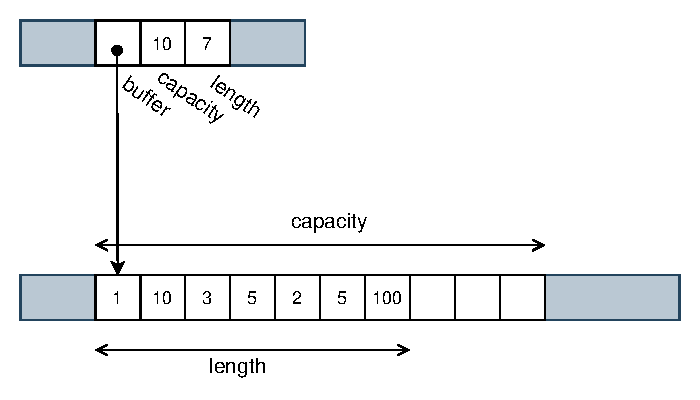
\includegraphics[width=5cm]{images/rust_vec.eps}
    \caption{Representation of Rust Vec$<$i32$>$}
    \label{fig:rustvec}
\end{figure}


\subsection{Move}
In Rust, for most types operations like assigning a value to a variable, passing it to a function, or returning it from a function do not copy the value: they move it. 
With move, a value can be transferred from one owner to another. The previous variable does not have ownership of the value; it is moved to a newly assigned variable. 
To understand how this assignment implementation is unique from other programing languages, Rust code example for Vec of strings are shown.

\begin{lstlisting}
    let s = vec!["lemon".to_string, 
                 "orange".to_string, 
                 "apple".to_string];
    let t = s;
    let u = s;
 \end{lstlisting}

The representation of the original Vec of String in Rust is the almost same in C++ vector of string. Figure~\ref{fig:rustvecmoved} however shows different behavior when Rust assigns s to t. 
The value is moved to t from s so that the source variable s is uninitialized. The Rust code actually throws compile error, because we are assigning uninitialized variable at the last line.

\begin{figure}[htb]
    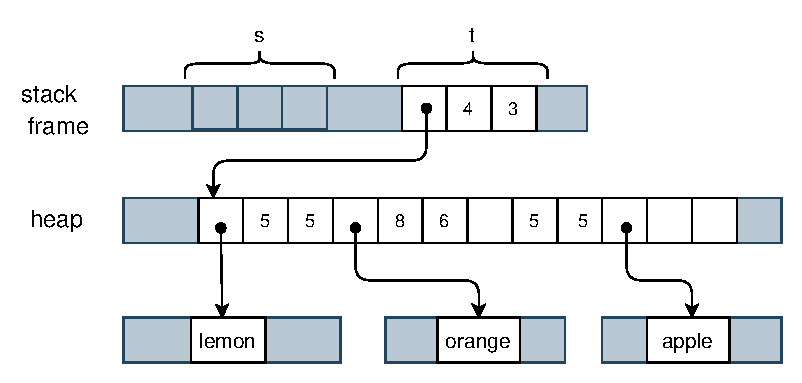
\includegraphics[width=5cm]{images/rust_vec_moved.eps}
    \caption{Representation of Rust Vec$<$String$>$ after assignment to another variable}
    \label{fig:rustvecmoved}
\end{figure}


\subsection{Borrowing}
Borrowing lets code use a value temporarily without affecting its ownership so that it reduces unnecessary movement of ownership. 
One use case is when value is used in function and needed to be passed to the argument. If the argument takes ownership and the function does not return the value, 
the ownership of value goes out of scope and the memory is deallocated. One can pass reference of the value to the argument instead of owner. 
The reference goes out of scope, but ownership remains the same.

\subsection{Type of Variable}
\label{sec:concept_diffval}
In Rust, there are three variable types: owner, reference, and slice (only for sequence of values). 
A developer is sometimes forced to use specific variable types. For example, some of methods are only implemented to specific variable types.
However, one can select any variable types for operation in most case.

These variables have different memory representation shown in Figure~\ref{fig:own_ref_slice}.
The owner has a pointer pointing to the memory address of sequence values, length of the values, and capacity allocated to store additional values. 
Reference and Slice are variables borrowing value owned by other variable. The reference is a pointer that points to the owner. 
The slice is a pointer that points to memory address of sequence values. It has value such as length of sequence values stored in the memory. 
Since they have different memory representation, an assumption is that it takes different time to access to the contents of the memory among these pointer types.
We examine this by constructing complex objects whose fields are these variable types. The details are explained in Section~\ref{sec:eval_diffval}.

\begin{figure}[htb]
    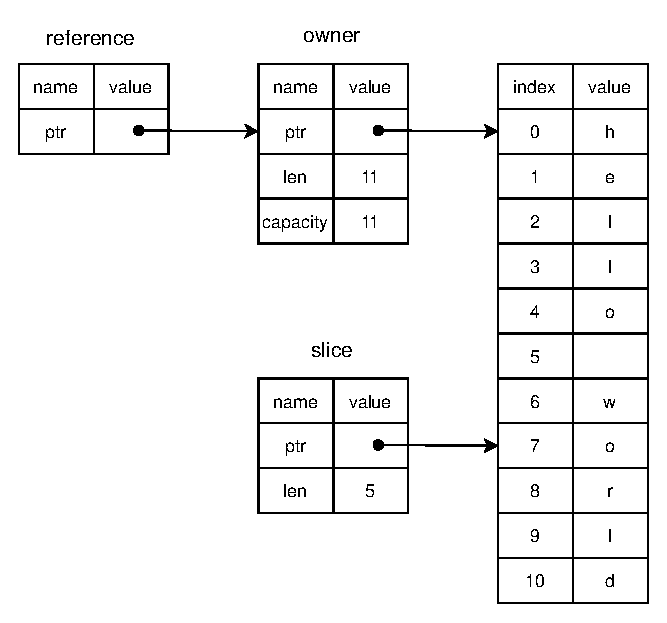
\includegraphics[width=5cm]{images/own_ref_slice.eps}
    \caption{Memory Representation of Owner, Reference, and Slice Type}
    \label{fig:own_ref_slice}
\end{figure}

\subsection{Reference Count}
\label{sec:concept_refcount}
Reference is useful to avoid movement of ownership. However, one needs to track its lifetime and explicitly includes it in code, 
because Rust compiler cannot infer it. This can be another encumbrance. We can instead acquire multiple owners to single value by using Reference Counting (Rc). 
By leveraging Rc, a value can be shared like what borrowing plays the role in Rust programming. 

The difference is that Rc checks number of owner pointing to the actual data and makes sure the data is not deleted 
until all the owners are dereferenced. Using Rc is sometimes preferable approach for developers especially when lifetime planning is extremely difficult.
However, the possible problems regarding to Rc are the cost for tracking the number of references and allocating memory on heap instead of stack.
Having these assumption, an experiment is conducted to examine difference of runtime performance of dropping reference and Rc. 

\subsection{Multithread}
\label{sec:concenpt_multithreading}
In Rust programming, writing concurrent code is relatively easy. The care Rust takes with reference, mutability, and lifetimes is valuable enough in single-threaded programs, 
but it also is in concurrent programming. Rust has tools to write concurrent code, such as threads, locks, atomic reference. 
One can implement various concurrent codes for the same purpose with different memory management strategies. 
The most ubiquitous tool used in Rust concurrent code is Atomic Reference Counting (Arc). 

Arc is a simple interface that allows threads to share data. Arc allows multiple variable to have ownerships of a particular value similarly to Rc, 
but also supports atomic feature enabling the ownerships exist in different threads. 
In many situation where developer write a multithreading code, the deletion of Arc happens significant amount of times. 
Similarly to Rc, our assumption is that deletion of Arc has also overhead when we compare to normal reference. 
To assess runtime performances of algorithm with Arc vs normal reference, we implement merge-sort algorithm in two different ways. 

\section{Conclusion}





\bibliographystyle{ACM-Reference-Format}
\bibliography{mybiblio.bib}


\end{document}
\endinput
